\chapter{User studies and Results}
\label{chap:results}

The results of this study were determined by the answers of a survey completed by the users that participate to the testing phase. \\
\noindent We recruited 6 people from Uppsala University and asked them to use the application for a period of 2 weeks and fill up a survey with 26 questions (see Appendix). The survey is anonymous and divided in 3 sections: the first part was designed to gather the information related to the audience. The second part aimed to rate the interest in learning a new language using a mobile device, whereas the third part was dedicated to the application itself. \\

\subsection*{Audience}
\label{sub:Audience}

This section presents the answers related to the users personal information to get a better understaning of the audience. From \ref{fig:gender_chart} and \ref{fig:age_chart} we can say that the majority of our users are male and between the age of 24-29 years old.  Table \ref{table:native_languages} describes the native language of the users.

\begin{figure}[!ht]
	\centering
	\begin{minipage}{.5\textwidth}
		\centering
		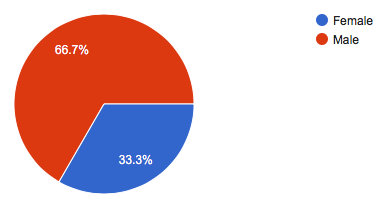
\includegraphics[scale=0.5]{Figures/responses/audience_gender.png}
		\caption{Gender chart}
		\label{fig:gender_chart}
	\end{minipage}%
	\begin{minipage}{.5\textwidth}
		\centering
		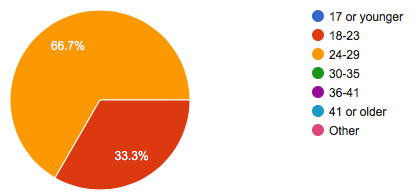
\includegraphics[scale=0.5]{Figures/responses/audience_age.png}
		\caption{Age chart}
		\label{fig:age_chart}
	\end{minipage}
\end{figure}

\begin{table}[!ht]
    \centering
    \begin{tabular}{|l|c|}
        \hline
        \multicolumn{1}{|c|}{\textbf{Native language}} & \textbf{Amount} \\ \hline
        Italian                                        & 2               \\ \hline
        Greek                                          & 2               \\ \hline
        Swedish                                        & 1               \\ \hline
        Arabic                                         & 1               \\ \hline
    \end{tabular}
    \caption{Users native languages}
    \label{table:native_languages}
\end{table}

\noindent All testers were students from the Computer Science department as well as comfortable in using mobile applications on a daily base.

\subsection*{Interest}
\label{sub:Interest}

This section describes the interest of our testers in learning and improving a new language using a mobile application instead of the traditional student-teacher class. Results are vey positive and we can confirm that the interest is high. In particular, avoiding the interaction with a physical teacher is very welcomed.

\begin{figure}[!ht]
	\centering
	\begin{minipage}{.5\textwidth}
		\centering
		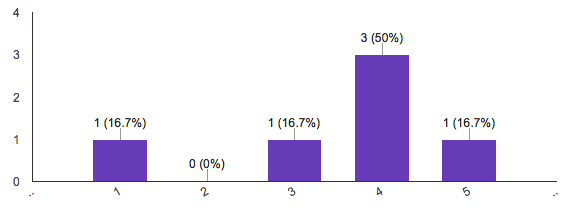
\includegraphics[scale=0.5]{Figures/responses/interest_improving_lang.png}
		\caption{Interest in improving English language}
		\label{fig:int_improving_lang}
	\end{minipage}%
	\begin{minipage}{.5\textwidth}
		\centering
		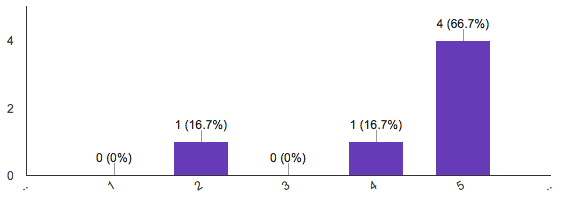
\includegraphics[scale=0.5]{Figures/responses/interest_learning_language.png}
		\caption{Interest in learning a new language}
		\label{fig:int_learnign_lang}
	\end{minipage}
    \begin{minipage}{.5\textwidth}
        \centering
        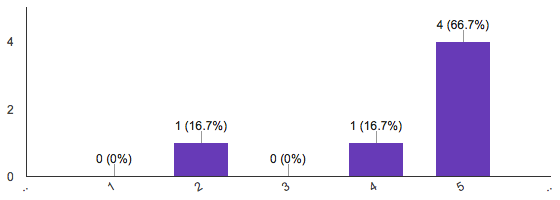
\includegraphics[scale=0.5]{Figures/responses/interest_usage_smartphone.png}
        \caption{Interest in using a smartphone}
        \label{fig:int_usage_smartphone}
    \end{minipage}%
\end{figure}
\begin{figure}[!ht]
	\centering
	\begin{minipage}{.5\textwidth}
		\centering
		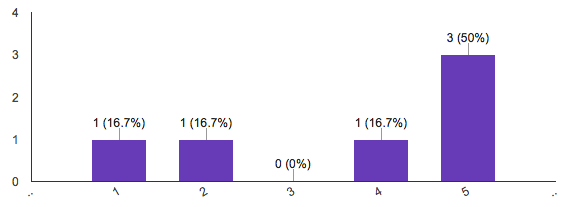
\includegraphics[scale=0.5]{Figures/responses/interest_visual_feedback.png}
		\caption{Interest in having visual feedback}
		\label{fig:int_visual_feedbak}
	\end{minipage}%
	\begin{minipage}{.5\textwidth}
		\centering
		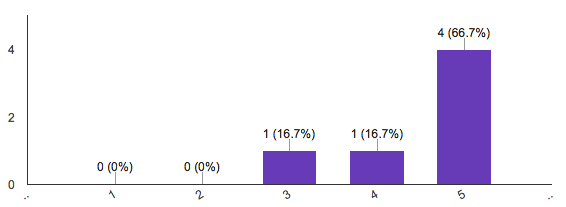
\includegraphics[scale=0.5]{Figures/responses/interest_no_teacher.png}
		\caption{Interest in not having a teacher's supervision}
		\label{fig:int_no_teacher}
	\end{minipage}
\end{figure}


\subsection*{Application}
\label{sub:Application}

\begin{figure}[!ht]
	\centering
	\begin{minipage}{.5\textwidth}
		\centering
		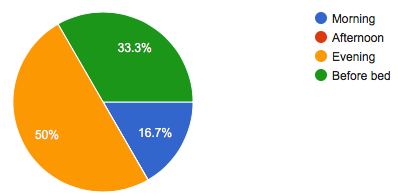
\includegraphics[scale=0.5]{Figures/responses/application_period_of_usage.png}
		\caption{Moment of the day}
		\label{fig:int_improving_lang}
	\end{minipage}%
	\begin{minipage}{.5\textwidth}
		\centering
		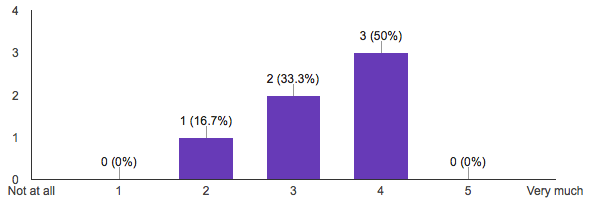
\includegraphics[scale=0.5]{Figures/responses/application_liked.png}
		\caption{General appreciation}
		\label{fig:int_usage_smartphone}
	\end{minipage}%
\end{figure}

\begin{figure}[!ht]
	\centering
	\begin{minipage}{.5\textwidth}
		\centering
		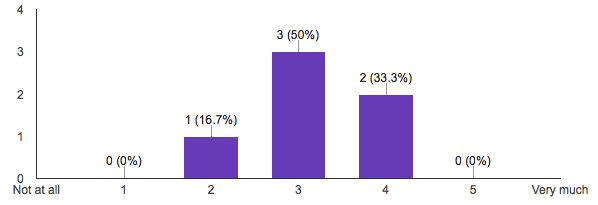
\includegraphics[scale=0.5]{Figures/responses/application_usage.png}
		\caption{Interest in continuing using the application}
		\label{fig:int_improving_lang}
	\end{minipage}%
	\begin{minipage}{.5\textwidth}
		\centering
		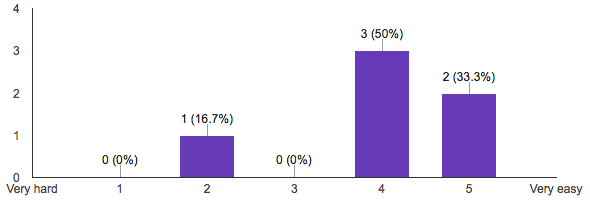
\includegraphics[scale=0.5]{Figures/responses/application_usage_difficulty.png}
		\caption{Usage difficulty}
		\label{fig:int_learnign_lang}
	\end{minipage}
\end{figure}

Here all the understandings

\begin{figure}[!ht]
	\centering
	\begin{minipage}{.5\textwidth}
		\centering
		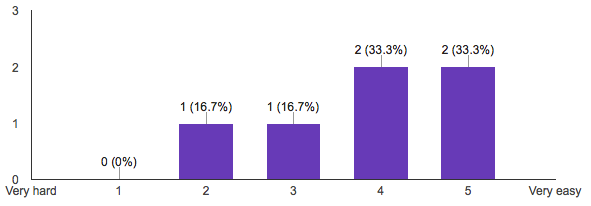
\includegraphics[scale=0.5]{Figures/responses/understanding_main.png}
		\caption{Understanding the main page}
		\label{fig:int_improving_lang}
	\end{minipage}%
	\begin{minipage}{.5\textwidth}
		\centering
		\includegraphics[scale=0.5]{Figures/responses/understanding_listening.png}
		\caption{Understanding the critical listening page}
		\label{fig:int_learnign_lang}
	\end{minipage}
	\begin{minipage}{.5\textwidth}
		\centering
		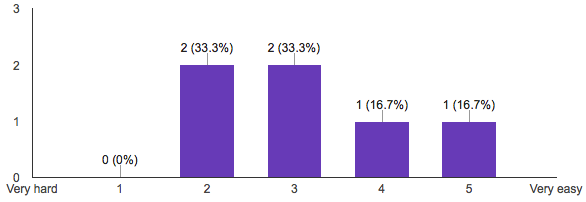
\includegraphics[scale=0.5]{Figures/responses/understanding_feedback.png}
		\caption{Understanding feedback page}
		\label{fig:int_usage_smartphone}
	\end{minipage}%
\end{figure}

\begin{figure}[!ht]
	\centering
	\begin{minipage}{.5\textwidth}
		\centering
		\includegraphics[scale=0.5]{Figures/responses/understanding_stress.png}
		\caption{Understanding stress on a sentence}
		\label{fig:int_improving_lang}
	\end{minipage}%
	\begin{minipage}{.5\textwidth}
		\centering
		\includegraphics[scale=0.5]{Figures/responses/understanding_pitch.png}
		\caption{Understanding pitch trend}
		\label{fig:int_learnign_lang}
	\end{minipage}
	\begin{minipage}{.5\textwidth}
		\centering
		\includegraphics[scale=0.5]{Figures/responses/understanding_vowels.png}
		\caption{Understanding vowels chart}
		\label{fig:int_usage_smartphone}
	\end{minipage}%
\end{figure}

\begin{figure}[!ht]
	\centering
	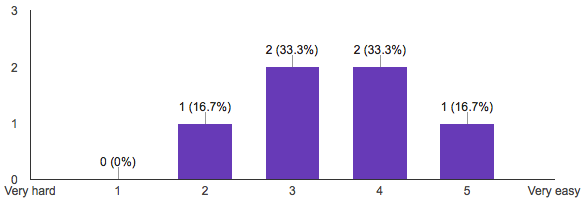
\includegraphics[scale=0.5]{Figures/responses/understanding_history.png}
	\caption{Understanding history page}
	\label{fig:int_improving_lang}
\end{figure}

Actual results

\begin{figure}[!ht]
	\centering
	\begin{minipage}{.5\textwidth}
		\centering
		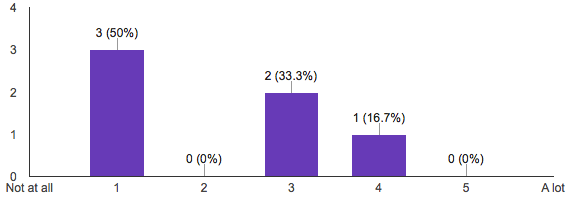
\includegraphics[scale=0.5]{Figures/responses/application_improved_pronunciation.png}
		\caption{Pronunciation improved}
		\label{fig:int_improving_lang}
	\end{minipage}%
	\begin{minipage}{.5\textwidth}
		\centering
		\includegraphics[scale=0.5]{Figures/responses/utility_of_listening.png}
		\caption{Utility of critical/self listening}
		\label{fig:int_learnign_lang}
	\end{minipage}
	\begin{minipage}{.5\textwidth}
		\centering
		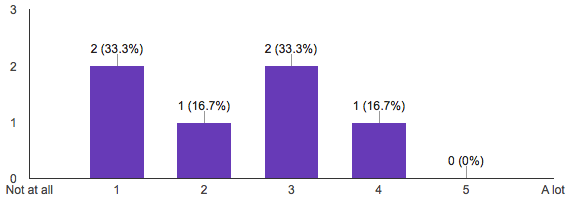
\includegraphics[scale=0.5]{Figures/responses/application_rate_feedback.png}
		\caption{Utility of feedback}
		\label{fig:int_usage_smartphone}
	\end{minipage}%
\end{figure}

\begin{figure}[!ht]
	\centering
	\includegraphics[scale=0.5]{Figures/responses/utility_of_history.png}
	\caption{Utility of history page}
	\label{fig:int_usage_smartphone}
\end{figure}%